% Use a package to avoid old (La)TeX habits.
\RequirePackage[l2tabu, orthodox]{nag}

% jsarticle: improved version of Japanese article style
% [dvipdfmx]: we use dvipdfmx.
% [uplatex]: we use uplatex.
% [papersize]: tell page size to pdf generator.
% [a4paper]: paper size is A4.
% [10pt]: point size is 10pt.
\documentclass[dvipdfmx,uplatex,papersize,a4paper,10pt]{jsarticle}

% This file is UTF-8 encoded.
\usepackage[utf8]{inputenc}
% Use T1 instead of OT1 for European texts.
\usepackage[T1]{fontenc}
% Fix Computer Modern rounding. Use this if you don't want to use Latin Modern.
% \usepackage{fix-cm}
% Use Latin Modern instead of Computer Modern font.
\usepackage{lmodern}

% AMS-related packages
\usepackage{amstext,amsmath,amsthm,amssymb,amsfonts}

% Avoid non-AMS mathematical usage.
\usepackage[all, warning]{onlyamsmath}

% Use otf fonts.
\usepackage{otf}
% Avoid "Font Shape undefined" error for italic Japanese texts.
\DeclareFontShape{JY2}{hmc}{m}{it}{<->ssub*hmc/m/n}{}
\DeclareFontShape{JY2}{hmc}{m}{sl}{<->ssub*hmc/m/n}{}
\DeclareFontShape{JY2}{hmc}{m}{sc}{<->ssub*hmc/m/n}{}
\DeclareFontShape{JY2}{hgt}{m}{it}{<->ssub*hgt/m/n}{}
\DeclareFontShape{JY2}{hgt}{m}{sl}{<->ssub*hgt/m/n}{}
\DeclareFontShape{JY2}{hmc}{bx}{it}{<->ssub*hgt/m/n}{}
\DeclareFontShape{JY2}{hmc}{bx}{sl}{<->ssub*hgt/m/n}{}
\DeclareFontShape{JT2}{hmc}{m}{it}{<->ssub*hmc/m/n}{}
\DeclareFontShape{JT2}{hmc}{m}{sl}{<->ssub*hmc/m/n}{}
\DeclareFontShape{JT2}{hmc}{m}{sc}{<->ssub*hmc/m/n}{}
\DeclareFontShape{JT2}{hgt}{m}{it}{<->ssub*hgt/m/n}{}
\DeclareFontShape{JT2}{hgt}{m}{sl}{<->ssub*hgt/m/n}{}
\DeclareFontShape{JT2}{hmc}{bx}{it}{<->ssub*hgt/m/n}{}
\DeclareFontShape{JT2}{hmc}{bx}{sl}{<->ssub*hgt/m/n}{}

% Use newtx fonts; maybe should be avoided in paper submissions.
\usepackage{newtxtext,newtxmath}

% Scale bigops in math. Not needed if we use newtxmath.
% \usepackage{exscale}

% \braket{}, \set{}
\usepackage{braket}

% Japanese Ruby generation.
\usepackage{pxrubrica}

% Syntax-highlighted program listings.
% jlisting: allow Japanese text in listings.
\usepackage{listings}

% Pass pagesize to DVI and configure page layout.
% [pass] is used to disable page layout overriding. Remove it if you want to configure page layout through this package.
% [dvipdfm] is for dvipdfmx.
% \usepackage[dvipdfm,pass]{geometry}

% Extended graphics package; provides \includegraphics.
\usepackage{graphicx}

% Extended color package; provides \color.
\usepackage{xcolor}

% Provides \url.
\usepackage{url}

% \mleft/\mright, a little clever replacements for \left/\right.
\usepackage{mleftright}

% \mathscr
\usepackage{mathrsfs}
% Override ursfs.fd to suppress "Font shape `U/rsfs/m/n' in size <5.5>/<10.5> not available" warning.
\DeclareFontFamily{U}{rsfs}{\skewchar\font127}
\DeclareFontShape{U}{rsfs}{m}{n}{%
  % <5> <6> rsfs5
  <5> <5.5> <6> rsfs5
  <7> rsfs7
  % <8> <9> <10> <10.95> <12> <14.4> <17.28> <20.74> <24.88> rsfs10
  <8> <9> <10> <10.5> <10.95> <12> <14.4> <17.28> <20.74> <24.88> rsfs10
}{}

% Part of hyperref.
\usepackage{nameref}

% Turns almost everything into hyper-reference.
\usepackage{hyperref}
% Improves non-ASCII characters in bookmarks.
\usepackage{pxjahyper}

% Float wrapper for algorithms.
\usepackage{algorithm}
% One of algorithm typesetting environments.
\usepackage{algpseudocode}

% Provides \cref, which automatically emits Lemma, Definition, etc.
\usepackage{cleveref}

\usepackage{tikz}
\usetikzlibrary{positioning,babel,arrows}

\theoremstyle{definition}
\newtheorem{definition}{定義}[section]
\newtheorem{example}[definition]{例}
\newtheorem{theorem}[definition]{定理}
\newtheorem{lemma}[definition]{補題}
\newtheorem{corollary}[definition]{系}
\newtheorem{proposition}[definition]{命題}
\newtheorem{axiom}[definition]{公理}
\newtheorem{remark}[definition]{注意}
\newtheorem{exercise}{練習問題}[section]

\crefname{definition}{定義}{定義}
\Crefname{definition}{定義}{定義}
\crefname{example}{例}{例}
\Crefname{example}{例}{例}
\crefname{theorem}{定理}{定理}
\Crefname{theorem}{定理}{定理}
\crefname{lemma}{補題}{補題}
\Crefname{lemma}{補題}{補題}
\crefname{corollary}{系}{系}
\Crefname{corollary}{系}{系}
\crefname{proposition}{命題}{命題}
\Crefname{proposition}{命題}{命題}
\crefname{axiom}{公理}{公理}
\Crefname{axiom}{公理}{公理}
\crefname{remark}{注意}{注意}
\Crefname{remark}{注意}{注意}
\crefname{exercise}{練習問題}{練習問題}
\Crefname{exercise}{練習問題}{練習問題}

\DeclareMathOperator{\id}{id}
\DeclareMathOperator{\Alg}{Alg}
\DeclareMathOperator{\Coalg}{Coalg}
\DeclareMathOperator{\RCA}{RCA}
\DeclareMathOperator{\CRA}{CRA}
\DeclareMathOperator{\Mono}{Mono}
\DeclareMathOperator{\Sub}{Sub}
\DeclareMathOperator{\true}{true}
\DeclareMathOperator{\op}{op}
\newcommand{\nexttime}{\mathop{\triangleright}}

\title{再帰的余代数いろいろ}
\author{原 将己}
%\date{2017年01月13日}

\begin{document}

\maketitle

\section{代数と余代数}

以下、 $\mathbf{C}$は圏とし、$F \colon \mathbf{C} \to \mathbf{C}$ は自己関手とする。

\begin{definition}[代数、余代数]

  $C$ の対象と射の組 $(A, \alpha)$ であって $\alpha \colon FA \to A$ となるものを \emph{$F$-代数 ($F$-algebra)} と呼ぶ。

  $C$ の対象と射の組 $(A, \alpha)$ であって $\alpha \colon A \to FA$ となるものを \emph{$F$-余代数 ($F$-coalgebra)} と呼ぶ。

  $F$-代数 $(A, \alpha)$ から $(B, \beta)$ への準同型とは、 $h \colon A \to B$ であって $\beta \circ Fh = h \circ \alpha$ となるもののことである。 $F$-代数とその準同型のなす圏を $\Alg(F)$ と書く。

  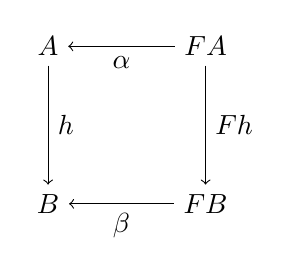
\begin{tikzpicture}[auto,every node/.style={on grid,node distance=2cm}]
    \node (A) {$A$};
    \node[right of=A] (FA) {$FA$};
    \node[below of=A] (B) {$B$};
    \node[right of=B] (FB) {$FB$};
    \draw[->] (FA) -- node {$\alpha$} (A);
    \draw[->] (FB) -- node {$\beta$} (B);
    \draw[->] (A) -- node {$h$} (B);
    \draw[->] (FA) -- node {$Fh$} (FB);
  \end{tikzpicture}

  $F$-余代数 $(A, \alpha)$ から $(B, \beta)$ への準同型とは、 $h \colon A \to B$ であって $\beta \circ h = Fh \circ \alpha$ となるもののことである。 $F$-余代数とその準同型のなす圏を $\Coalg(F)$ と書く。

  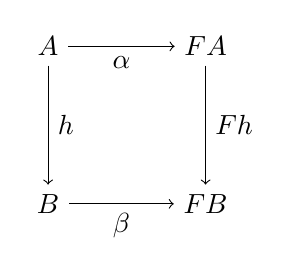
\begin{tikzpicture}[auto,every node/.style={on grid,node distance=2cm}]
    \node (A) {$A$};
    \node[right of=A] (FA) {$FA$};
    \node[below of=A] (B) {$B$};
    \node[right of=B] (FB) {$FB$};
    \draw[->] (A) -- node[swap] {$\alpha$} (FA);
    \draw[->] (B) -- node[swap] {$\beta$} (FB);
    \draw[->] (A) -- node {$h$} (B);
    \draw[->] (FA) -- node {$Fh$} (FB);
  \end{tikzpicture}
\end{definition}

\begin{definition}[余代数-代数準同型]
  $F$-余代数 $(A, \alpha)$ から $F$-代数 $(B, \beta)$ への\emph{余代数-代数準同型 (coalgebra-to-algebra homomorphism)} とは、 $h \colon A \to B$ であって、 $\beta \circ Fh \circ \alpha = h$ となるもののことである。

  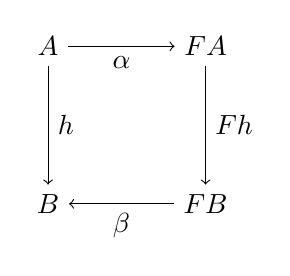
\begin{tikzpicture}[auto,every node/.style={on grid,node distance=2cm}]
    \node (A) {$A$};
    \node[right of=A] (FA) {$FA$};
    \node[below of=A] (B) {$B$};
    \node[right of=B] (FB) {$FB$};
    \draw[->] (A) -- node[swap] {$\alpha$} (FA);
    \draw[->] (FB) -- node {$\beta$} (B);
    \draw[->] (A) -- node {$h$} (B);
    \draw[->] (FA) -- node {$Fh$} (FB);
  \end{tikzpicture}
\end{definition}

\begin{definition}[始代数と終余代数]
  $\Alg(F)$ の始対象を\emph{始代数 (initial algera)}という。$\Coalg(F)$ の終対象を\emph{終余代数 (terminal coalgebra, final coalgebra)}という。

  定義より、始代数と終余代数は(存在するならば)同型を除いて一意である。
\end{definition}

\begin{definition}[再帰的余代数と余再帰的代数]~\cite{MR0364389},~\cite{DBLP:conf/sbmf/CaprettaUV09}

  余代数であって、任意の代数への準同型が一意に存在するものを\emph{再帰的$F$-余代数 (recursive $F$-coalgebra)}という。本資料では再帰的余代数からなる$\Coalg(F)$の充満部分圏を$\RCA(F)$と表記する。

  代数であって、任意の余代数からの準同型が一意に存在するものを\emph{余再帰的$F$-代数 (corecursive $F$-algebra)}という。本資料では余再帰的代数からなる$\Alg(F)$の充満部分圏を$\CRA(F)$と表記する。
\end{definition}

\begin{remark}
  再帰的余代数と始代数の普遍性は良く似ている。実際、 $\alpha$ が可逆のとき、この2つの定義は ($\alpha$ の向きを互いに逆にすることで) 同値になる。

  同様に、余再帰的代数と終余代数の定義も、 $\alpha$ が可逆のときに同値になる。
\end{remark}

\section{Lambekの定理}

\begin{theorem}[Lambek]
  始代数 $(A, \alpha)$ の $\alpha$ は常に可逆である。双対的に、終余代数も可逆である。
\end{theorem}

\begin{proof}
  始代数について示す。 $(A, \alpha)$ を始代数とする。このとき $(FA, F\alpha)$ も代数だから、代数の準同型 ($h \colon A \to FA$ であって $F\alpha \circ Fh = h \circ \alpha$ となるもの)が存在する。

  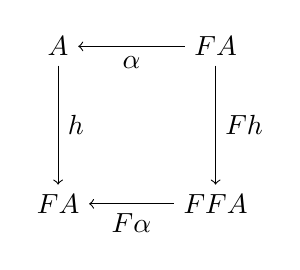
\begin{tikzpicture}[auto,every node/.style={on grid,node distance=2cm}]
    \node (A) {$A$};
    \node[right of=A] (FA) {$FA$};
    \node[below of=A] (FA2) {$FA$};
    \node[right of=FA2] (FFA2) {$FFA$};
    \draw[->] (FA) -- node {$\alpha$} (A);
    \draw[->] (FFA2) -- node {$F\alpha$} (FA2);
    \draw[->] (A) -- node {$h$} (FA2);
    \draw[->] (FA) -- node {$Fh$} (FFA2);
  \end{tikzpicture}

  $h$ も $\alpha$ も代数の準同型だから、 $\alpha \circ h$ は $(A, \alpha)$ の自己準同型である。一方、 $\id_A$ も $(A, \alpha)$ の自己準同型である。始代数からの準同型は一意だから、 $\alpha \circ h = \id_A$ である。

  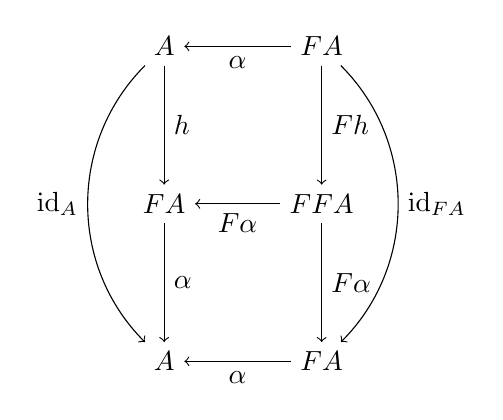
\begin{tikzpicture}[auto,every node/.style={on grid,node distance=2cm}]
    \node (A) {$A$};
    \node[right of=A] (FA) {$FA$};
    \node[below of=A] (FA2) {$FA$};
    \node[right of=FA2] (FFA2) {$FFA$};
    \node[below of=FA2] (A3) {$A$};
    \node[right of=A3] (FA3) {$FA$};
    \draw[->] (FA) -- node {$\alpha$} (A);
    \draw[->] (FFA2) -- node {$F\alpha$} (FA2);
    \draw[->] (FA3) -- node {$\alpha$} (A3);
    \draw[->] (A) -- node {$h$} (FA2);
    \draw[->] (FA) -- node {$Fh$} (FFA2);
    \draw[->] (FA2) -- node {$\alpha$} (A3);
    \draw[->] (FFA2) -- node {$F\alpha$} (FA3);
    \draw[->] (A) to[bend right=45] node[swap] {$\id_A$} (A3);
    \draw[->] (FA) to[bend left=45] node {$\id_{FA}$} (FA3);
  \end{tikzpicture}

  $\alpha \circ h = \id_A$ と $h$ の準同型性により、 $h \circ \alpha = F\alpha \circ Fh = F\id_A = \id_{FA}$ である。

  したがって、 $h$ は $\alpha$ の逆射である。
\end{proof}

\begin{corollary}
  始代数(の逆射)は再帰的余代数である。双対的に、終余代数(の逆射)は余再帰的代数である。
\end{corollary}

\begin{theorem}
  始代数(の逆射)は$\RCA(F)$の終対象である。双対的に、終余代数(の逆射)は$\CRA(F)$の始対象である。
\end{theorem}

\begin{proof}
  $(A, \alpha)$ を始代数とする。このとき $(A, \alpha^{-1})$が$\RCA(F)$の終対象であることを示す。

  $(B, \beta) \in \RCA(F)$ とする。 $(B, \beta)$ から $(A, \alpha^{-1})$ への代数準同型は、$(B, \beta)$ から $(A, \alpha)$ への余代数-代数準同型に他ならない。したがって $B$ の再帰性から、代数準同型は一意である。

  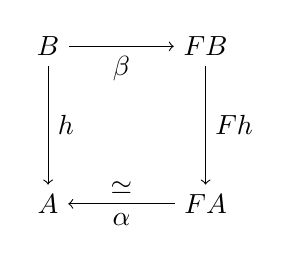
\begin{tikzpicture}[auto,every node/.style={on grid,node distance=2cm}]
    \node (A) {$A$};
    \node[right of=A] (FA) {$FA$};
    \node[above of=A] (B) {$B$};
    \node[right of=B] (FB) {$FB$};
    \draw[->] (FA) -- node {$\alpha$} node[swap] {$\simeq$} (A);
    \draw[->] (B) -- node[swap] {$\beta$} (FB);
    \draw[->] (B) -- node {$h$} (A);
    \draw[->] (FB) -- node {$Fh$} (FA);
  \end{tikzpicture}
\end{proof}

\section{逆Lambekの定理}

(逆Lambekという名前は本資料に固有である。)

\begin{lemma}
  $(A, \alpha)$ が再帰的余代数であるとき、 $(FA, F\alpha)$ も再帰的余代数である。双対的に、 $(A, \alpha)$ が余再帰的代数であるとき、 $(FA, F\alpha)$ も余再帰的代数である。
\end{lemma}

\begin{proof}
  $(A, \alpha)$ を再帰的余代数とし、 $(B, \beta)$ を代数とする。

  $A$ の再帰性より、 $A$ から $B$ への余代数-代数準同型 ($h \colon A \to B$ であって $\beta \circ Fh \circ \alpha = h$ となるもの) が一意に存在する。これを用いて $f = \beta \circ Fh$ と定義する。

  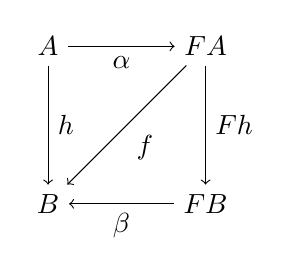
\begin{tikzpicture}[auto,every node/.style={on grid,node distance=2cm}]
    \node (A) {$A$};
    \node[right of=A] (FA) {$FA$};
    \node[below of=A] (B) {$B$};
    \node[right of=B] (FB) {$FB$};
    \draw[->] (A) -- node[swap] {$\alpha$} (FA);
    \draw[->] (FB) -- node {$\beta$} (B);
    \draw[->] (A) -- node {$h$} (B);
    \draw[->] (FA) -- node {$Fh$} (FB);
    \draw[->] (FA) -- node {$f$} (B);
  \end{tikzpicture}

  この $f$ は $\beta \circ Ff \circ F\alpha = \beta \circ F(\beta \circ Fh \circ \alpha) = \beta \circ Fh = f$ を満たす。したがって $f$ は $FA$ から $B$ への余代数-代数準同型である。

  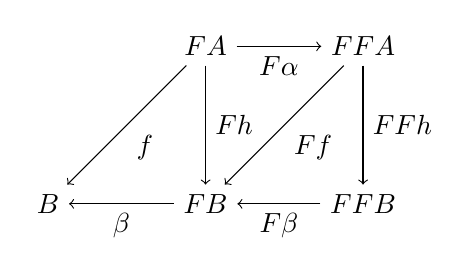
\begin{tikzpicture}[auto,every node/.style={on grid,node distance=2cm}]
    %\node (A) {$A$};
    \node (A) {};
    \node[right of=A] (FA) {$FA$};
    \node[right of=FA] (FFA) {$FFA$};
    \node[below of=A] (B) {$B$};
    \node[right of=B] (FB) {$FB$};
    \node[right of=FB] (FFB) {$FFB$};
    %\draw[->] (A) -- node[swap] {$\alpha$} (FA);
    \draw[->] (FA) -- node[swap] {$F\alpha$} (FFA);
    \draw[->] (FB) -- node {$\beta$} (B);
    \draw[->] (FFB) -- node {$F\beta$} (FB);
    %\draw[->] (A) -- node {$h$} (B);
    \draw[->] (FA) -- node {$Fh$} (FB);
    \draw[->] (FFA) -- node {$FFh$} (FFB);
    \draw[->] (FA) -- node {$f$} (B);
    \draw[->] (FFA) -- node {$Ff$} (FB);
  \end{tikzpicture}

  逆に $f' \colon FA \to B$ が $\beta \circ Ff' \circ F\alpha = f'$ を満たすとする。 $h' = f' \circ \alpha$ とおくと、 $\beta \circ Fh' \circ \alpha = \beta \circ Ff' \circ F\alpha \circ \alpha = f' \circ \alpha = h'$ となるから、 $h'$ は $A$ から $B$ への余代数-代数準同型である。

  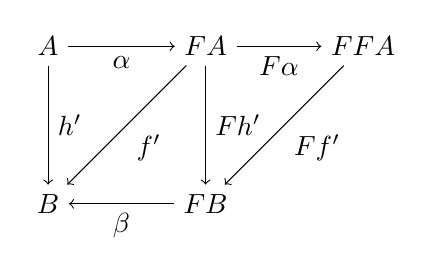
\begin{tikzpicture}[auto,every node/.style={on grid,node distance=2cm}]
    \node (A) {$A$};
    \node[right of=A] (FA) {$FA$};
    \node[right of=FA] (FFA) {$FFA$};
    \node[below of=A] (B) {$B$};
    \node[right of=B] (FB) {$FB$};
    %\node[right of=FB] (FFB) {$FFB$};
    \draw[->] (A) -- node[swap] {$\alpha$} (FA);
    \draw[->] (FA) -- node[swap] {$F\alpha$} (FFA);
    \draw[->] (FB) -- node {$\beta$} (B);
    %\draw[->] (FFB) -- node {$F\beta$} (FB);
    \draw[->] (A) -- node {$h'$} (B);
    \draw[->] (FA) -- node {$Fh'$} (FB);
    %\draw[->] (FFA) -- node {$FFh'$} (FFB);
    \draw[->] (FA) -- node {$f'$} (B);
    \draw[->] (FFA) -- node {$Ff'$} (FB);
  \end{tikzpicture}

  $A$ の再帰性から $h' = h$ となる。したがって、 $f' = \beta \circ Ff' \circ F\alpha = \beta \circ Fh' = \beta \circ Fh = f$ となる。

  以上より $FA$ から $B$ への余代数-代数準同型は一意に存在する。したがって、 $(FA, F\alpha)$ は再帰的余代数である。
\end{proof}

\begin{theorem}[逆Lambek]
  $\RCA(F)$ の終対象は可逆である。双対的に、 $\CRA(F)$ の始対象は可逆である。
\end{theorem}

\begin{proof}
  $(A, \alpha)$ を $\RCA(F)$ の終対象とする。$(FA, F\alpha)$ も再帰的余代数だから、 $(A, \alpha)$ の終性より、$FA$ から $A$ への余代数準同型 ($h \colon FA \to A$ であって $\alpha \circ h = Fh \circ F\alpha$ となるもの) が存在する。

  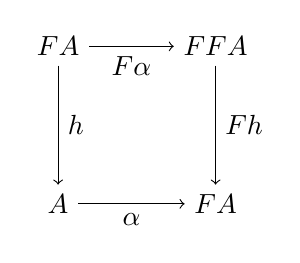
\begin{tikzpicture}[auto,every node/.style={on grid,node distance=2cm}]
    \node (A) {$A$};
    \node[right of=A] (FA) {$FA$};
    \node[above of=A] (FA2) {$FA$};
    \node[right of=FA2] (FFA2) {$FFA$};
    \draw[->] (A) -- node[swap] {$\alpha$} (FA);
    \draw[->] (FA2) -- node[swap] {$F\alpha$} (FFA2);
    \draw[->] (FA2) -- node {$h$} (A);
    \draw[->] (FFA2) -- node {$Fh$} (FA);
  \end{tikzpicture}

  $h$ も $\alpha$ も余代数の準同型だから、 $h \circ \alpha$ は $(A, \alpha)$ の自己準同型である。一方、 $\id_A$ も $(A, \alpha)$ の自己準同型である。終再帰的余代数への準同型は一意だから、 $h \circ \alpha = \id_A$ である。

  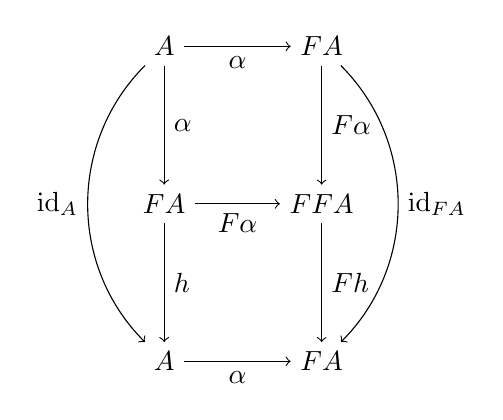
\begin{tikzpicture}[auto,every node/.style={on grid,node distance=2cm}]
    \node (A) {$A$};
    \node[right of=A] (FA) {$FA$};
    \node[above of=A] (FA2) {$FA$};
    \node[right of=FA2] (FFA2) {$FFA$};
    \node[above of=FA2] (A3) {$A$};
    \node[right of=A3] (FA3) {$FA$};
    \draw[->] (A) -- node[swap] {$\alpha$} (FA);
    \draw[->] (FA2) -- node[swap] {$F\alpha$} (FFA2);
    \draw[->] (A3) -- node[swap] {$\alpha$} (FA3);
    \draw[->] (FA2) -- node {$h$} (A);
    \draw[->] (FFA2) -- node {$Fh$} (FA);
    \draw[->] (A3) -- node {$\alpha$} (FA2);
    \draw[->] (FA3) -- node {$F\alpha$} (FFA2);
    \draw[->] (A3) to[bend right=45] node[swap] {$\id_A$} (A);
    \draw[->] (FA3) to[bend left=45] node {$\id_{FA}$} (FA);
  \end{tikzpicture}

  $h \circ \alpha = \id_A$ と $h$ の準同型性により、 $\alpha \circ h = Fh \circ F\alpha = F\id_A = \id_{FA}$ である。

  したがって、 $h$ は $\alpha$ の逆射である。
\end{proof}

\begin{corollary}
  $\RCA(F)$ の終対象(の逆射)は始代数である。双対的に、$\CRA(F)$ の始対象(の逆射)は終余代数である。
\end{corollary}

\section{完備束}

\begin{definition}[完備束と完備半束]
  $(A, \leq)$ を半順序集合とする。

  \begin{itemize}
    \item $X \subseteq A$ について、 $y \in A$ が $X$ の交わり (meet) であるとは、以下を満たすことである。
      \begin{itemize}
        \item 任意の $x \in X$ に対して、 $y \leq x$ である。
        \item 任意の $z \in A$ について、これが任意の $x \in X$ に対して $z \leq x$ を満たすなら、 $z \leq y$ である。
      \end{itemize}

      交わりは存在すれば一意であり、これを $\bigwedge X$ と書く。

    \item 双対的に、 $X \subseteq A$ について、 $y \in A$ が $X$ の結び (join) であるとは、以下を満たすことである。
      \begin{itemize}
        \item 任意の $x \in X$ に対して、 $x \leq y$ である。
        \item 任意の $z \in A$ について、これが任意の $x \in X$ に対して $x \leq z$ を満たすなら、 $y \leq z$ である。
      \end{itemize}

      結びは存在すれば一意であり、これを $\bigvee X$ と書く。

    \item $A$ が\emph{完備交わり半束 (complete meet-semilattice)}であるとは、$A$ が任意の部分集合の交わりを持つことである。
    \item $A$ が\emph{完備結び半束 (complete join-semilattice)}であるとは、$A$ が任意の部分集合の結びを持つことである。
    \item $A$ が\emph{完備束 (complete lattice)}であるとは、 $A$ が完備交わり半束かつ完備結び半束であることである。
  \end{itemize}
\end{definition}

\begin{theorem}
  以下は同値:
  \begin{itemize}
    \item $A$ は完備交わり半束である。
    \item $A$ は完備結び半束である。
    \item $A$ は完備束である。
  \end{itemize}
\end{theorem}

\begin{proof}
  $A$ が完備交わり半束ならば完備結び半束であることを示す。逆は双対的に示される。残りの含意は自明である。

  $A$ を完備交わり半束とする。 $X \subseteq A$ とする。$X$ の上界を集めた集合を $\mathop{\uparrow} X$ とおく。 $\bigwedge \mathop{\uparrow} X$ が $X$ の結びであることを示す。

  $x \in X$ とする。$\mathop{\uparrow} X$ の定義から、任意の $y \in \mathop{\uparrow} X$ に対し、 $x \leq y$ である。$\bigwedge$ の定義から、 $x \in \bigwedge \mathop{\uparrow} X$ である。

  $z \in A$ を $X$ の上界とする。このとき $z \in \mathop{\uparrow} X$ である。 $\bigwedge$ の定義から、 $\bigwedge \mathop{\uparrow} X \leq z$ である。

  以上により、 $\bigwedge \mathop{\uparrow} X$ は $X$ の結びである。
\end{proof}

\begin{definition}[不動点]
  順序集合における代数を\emph{前不動点 (pre-fixed point)}という。

  順序集合における余代数を\emph{後不動点 (post-fixed point)}という。

  代数または余代数で、可逆なものを\emph{不動点 (fixed point)}という。

  始代数を\emph{最小不動点 (least fixed point)}という。(Lambekの定理より、これは不動点である。)

  終余代数を\emph{最大不動点 (greatest fixed point)}という。(Lambekの定理より、これは不動点である。)
\end{definition}

\begin{theorem}[Knaster-Tarski]
  $(A, \leq)$ を完備束とし、 $f \colon A \to A$ を単調写像(順序集合間の関手)とする。このとき、このとき、 $f$は最小不動点と最大不動点を持つ。

  (より一般に、不動点の集合が再び完備束となることが知られているが、ここでは上の事実のみ使う。)
\end{theorem}

\begin{proof}
  全ての前不動点の交わりを $\mu f$ とおく。 $\mu f$もまた前不動点である。したがって $\mu f$ の定義より、これは始代数(最小不動点)である。
\end{proof}

\section{部分対象}

\begin{definition}[部分対象の擬順序集合]
  $A \in \mathbf{C}$ とする。 $A$ の\emph{部分対象 (subobject)}とは、 $\mathbf{C}$ の対象と射の組 $(I, i)$ であって、 $i \colon I \hookrightarrow A$ となるものである。($\hookrightarrow$ はmono射であることを意味する。)

  スライス圏 $\mathbf{C}/A$ を $A$ の部分対象に制限した充満部分圏を $\Mono(A)$ と書く。
\end{definition}

\begin{theorem}
  $\Mono(A)$ は擬順序クラスである。
\end{theorem}

\begin{proof}
  どの並行射も等しいことは、mono射の性質から導かれる。
\end{proof}

\begin{definition}[部分対象の順序集合]
  $\Mono(A)$ を同値類で割って順序集合としたものを $\Sub(A)$ と書く。
\end{definition}

\begin{definition}[整羃圏]
  全ての $A \in \mathbf{C}$ について、 $\Sub(A)$ が小さい (真クラスではなく、集合である) とき、 $\mathbf{C}$ は\emph{整羃 (well-powered)}であるという。
\end{definition}

\begin{definition}[初等トポス]
  $\mathbf{C}$ の\emph{部分対象分類子 (subobject classifier)}とは、 $\mathbf{C}$ の対象と射の組 $(\Omega, \true)$ であって、以下の条件を満たすものである。
  \begin{itemize}
    \item $\true \colon 1 \to \Omega$ である。ただし、 $1 \in \mathbf{C}$ は $\mathbf{C}$ の終対象とする。
    \item 任意の $I, A \in \mathbf{C}$, $i \colon I \hookrightarrow A$ に対し、以下の図式 \\
      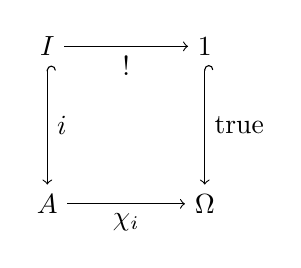
\begin{tikzpicture}[auto,every node/.style={on grid,node distance=2cm}]
        \node (A) {$A$};
        \node[above of=A] (I) {$I$};
        \node[right of=A] (Omega) {$\Omega$};
        \node[above of=Omega] (One) {$1$};
        \draw[right hook->] (I) -- node {$i$} (A);
        \draw[right hook->] (One) -- node {$\true$} (Omega);
        \draw[->] (A) -- node[swap] {$\chi_i$} (Omega);
        \draw[->] (I) -- node[swap] {$!$} (One);
      \end{tikzpicture} \\
      を引き戻しとして成立させるような $\chi_i$ がただ1つ存在する。ただし、 $! \colon I \to 1$ は終対象に対する唯一の射のこととする。
  \end{itemize}

  $\mathbf{C}$ が\emph{初等トポス (elementary topos)}、あるいは単に\emph{トポス (topos)}であるとは、 $\mathbf{C}$ が有限極限と指数対象と部分対象分類子を持つことである。
\end{definition}

\begin{example}
  $\mathbf{Set}$ はトポスである。より一般に、 $[\mathbf{I}, \mathbf{Set}]$ もトポスである。 $\mathbf{Set}$ を有限集合に限定したものもトポスである。
\end{example}

\begin{theorem}
  $\mathbf{C}$ がトポスであるとき、これが局所小であることと整羃であることは同値である。
\end{theorem}

\begin{proof}
  略
\end{proof}

\begin{theorem}
  $\mathbf{C}$ が完備で局所小なトポスであるとき、任意の $A \in \mathbf{C}$ に対し、 $\Sub(A)$ は完備束である。
\end{theorem}

\begin{proof}
  $\mathbf{C}$ が完備だから、 $\mathbf{C}/A$ も小極限を持つ。忠実充満関手は極限を反映するから、 $\Sub(A)$ も小極限を持つ。 $\mathbf{C}$ が整羃である、すなわち $\Sub(A)$ が小さいことから、 $\Sub(A)$ は順序集合の意味で完備 (交わり完備半束) であることがわかる。したがって、 $\Sub(A)$ は完備束である。
\end{proof}

\begin{definition}[逆像]
  $f \colon B \to A$, $i \colon I \hookrightarrow A$ とするとき、以下の引き戻し \\
  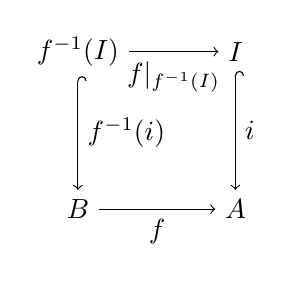
\begin{tikzpicture}[auto,every node/.style={on grid,node distance=2cm}]
    \node (A) {$A$};
    \node[above of=A] (I) {$I$};
    \node[left of=A] (B) {$B$};
    \node[above of=B] (InvImg) {$f^{-1}(I)$};
    \draw[right hook->] (I) -- node {$i$} (A);
    \draw[right hook->] (InvImg) -- node {$f^{-1}(i)$} (B);
    \draw[->] (B) -- node[swap] {$f$} (A);
    \draw[->] (InvImg) -- node[swap] {$f|_{f^{-1}(I)}$} (I);
  \end{tikzpicture} \\
  を$I$の$f$による\emph{逆像 (inverse image)}と呼ぶ。
\end{definition}

\section{整礎余代数}

整礎余代数について議論するときは、以下を仮定する。

\begin{itemize}
  \item $\mathbf{C}$ は圏である。
  \item $F \colon \mathbf{C} \to \mathbf{C}$ は自己関手である。
  \item $\mathbf{C}$ は逆像を持つ。
  \item $F$ はmono射をmono射に写す。
  \item $F$ は逆像を逆像に写す。
\end{itemize}

\begin{definition}[整礎余代数]
  $(A, \alpha)$ を $F$-余代数とし、 $(I, i)$ を $A$ の部分対象とする。以下の引き戻し図式 \\
  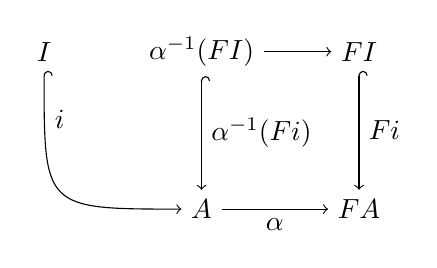
\begin{tikzpicture}[auto,every node/.style={on grid,node distance=2cm}]
    \node (A) {$A$};
    \node[right of=A] (FA) {$FA$};
    \node[above of=FA] (FI) {$FI$};
    \node[above of=A] (InvImg) {$\alpha^{-1}(FI)$};
    \node[left of=A] (Ibelow) {};
    \node[above of=Ibelow] (I) {$I$};
    \draw[right hook->] (FI) -- node {$Fi$} (FA);
    \draw[right hook->] (InvImg) -- node {$\alpha^{-1}(Fi)$} (A);
    \draw[right hook->] (I) .. controls (Ibelow) .. node[pos=0.2] {$i$} (A);
    \draw[->] (A) -- node[swap] {$\alpha$} (FA);
    \draw[->] (InvImg) -- node[swap] {} (FI);
  \end{tikzpicture} \\
  において、 $\alpha^{-1}(Fi)$ が $i$ を経由する、すなわち \\
  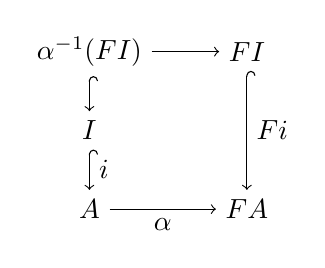
\begin{tikzpicture}[auto,every node/.style={on grid,node distance=2cm}]
    \node (A) {$A$};
    \node[right of=A] (FA) {$FA$};
    \node[above of=FA] (FI) {$FI$};
    \node[above of=A] (InvImg) {$\alpha^{-1}(FI)$};
    \node[above=1cm of A] (I) {$I$};
    \draw[right hook->] (FI) -- node {$Fi$} (FA);
    \draw[right hook->] (InvImg) -- node {} (I);
    \draw[right hook->] (I) -- node {$i$} (A);
    \draw[->] (A) -- node[swap] {$\alpha$} (FA);
    \draw[->] (InvImg) -- node[swap] {} (FI);
  \end{tikzpicture} \\
  となるとき、 $(I, i)$ は帰納的 (inductive) であるという。

  帰納的な部分対象が $(A, \id_A)$ と同型なものに限られる (すなわち、 $(I, i)$ が帰納的なら $i$ が可逆である) とき、 $(A, \alpha)$ は\emph{整礎 (well-founded)}であるという。
\end{definition}

\begin{definition}[反礎代数]
  双対的に、 $F$-代数 $(A, \alpha)$ が $\mathbf{C}^{\op}$ で整礎余代数であるとき、 $(A, \alpha)$ を\emph{反礎代数 (anti-founded algebra)}という。
\end{definition}

\begin{theorem}~\cite{DBLP:books/daglib/0031002}
  $\mathbf{C}$ が完備で局所小なトポスであるとき、 $\mathbf{C}$ の再帰的余代数は整礎余代数である。
\end{theorem}

\begin{proof}
  $(A, \alpha)$ を 再帰的 $F$-余代数とする。

  関数 $\nexttime \colon \Sub(A) \to \Sub(A)$ を、 $\nexttime(I) = \alpha^{-1}(FI)$ と定義すると、これは単調写像になっている。 $\Sub(A)$ は完備束だから、 $\nexttime$ の最小不動点が存在する。これを $(I, i)$ とおく。

  $(I, i)$ が $\nexttime$ の不動点であるというのは、すなわち \\
  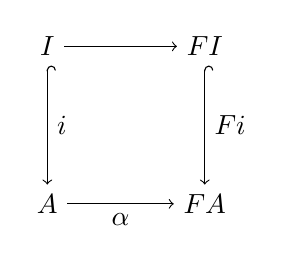
\begin{tikzpicture}[auto,every node/.style={on grid,node distance=2cm}]
    \node (A) {$A$};
    \node[right of=A] (FA) {$FA$};
    \node[above of=FA] (FI) {$FI$};
    \node[above of=A] (I) {$I$};
    \draw[right hook->] (FI) -- node {$Fi$} (FA);
    \draw[right hook->] (I) -- node {$i$} (A);
    \draw[->] (A) -- node[swap] {$\alpha$} (FA);
    \draw[->] (I) -- node[swap] {} (FI);
  \end{tikzpicture} \\
  という引き戻し図式が存在することに他ならない。

  さらに、 $\mathbf{C}$ はトポスであるから、以下の引き戻し図式 \\
  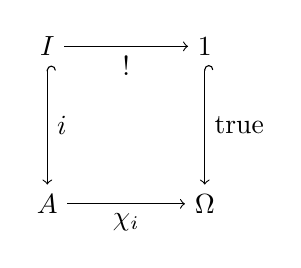
\begin{tikzpicture}[auto,every node/.style={on grid,node distance=2cm}]
    \node (A) {$A$};
    \node[above of=A] (I) {$I$};
    \node[right of=A] (Omega) {$\Omega$};
    \node[above of=Omega] (One) {$1$};
    \draw[right hook->] (I) -- node {$i$} (A);
    \draw[right hook->] (One) -- node {$\true$} (Omega);
    \draw[->] (A) -- node[swap] {$\chi_i$} (Omega);
    \draw[->] (I) -- node[swap] {$!$} (One);
  \end{tikzpicture} \\
  が存在する。 $F$ は逆像図式を保存すると仮定しているから、上の図式を \\
  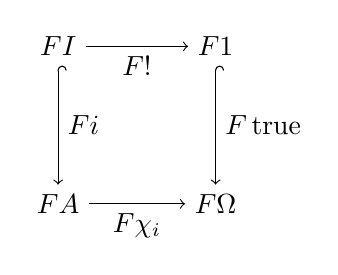
\begin{tikzpicture}[auto,every node/.style={on grid,node distance=2cm}]
    \node (FA) {$FA$};
    \node[above of=FA] (FI) {$FI$};
    \node[right of=FA] (FOmega) {$F\Omega$};
    \node[above of=FOmega] (FOne) {$F1$};
    \draw[right hook->] (FI) -- node {$Fi$} (FA);
    \draw[right hook->] (FOne) -- node {$F\true$} (FOmega);
    \draw[->] (FA) -- node[swap] {$F\chi_i$} (FOmega);
    \draw[->] (FI) -- node[swap] {$F!$} (FOne);
  \end{tikzpicture} \\
  と持ち上げても、引き戻し図式となる。これらを連結し、さらに $\chi_{F\true}$ を定義する図式を繋げると \\
  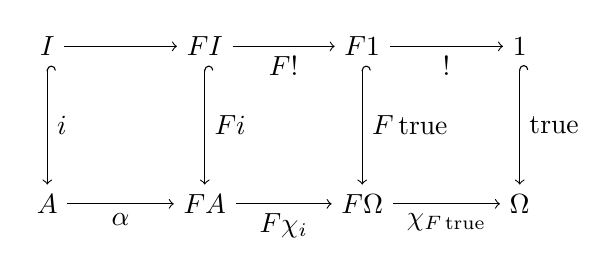
\begin{tikzpicture}[auto,every node/.style={on grid,node distance=2cm}]
    \node (A) {$A$};
    \node[right of=A] (FA) {$FA$};
    \node[above of=FA] (FI) {$FI$};
    \node[above of=A] (I) {$I$};
    \node[right of=FA] (FOmega) {$F\Omega$};
    \node[above of=FOmega] (FOne) {$F1$};
    \node[right of=FOmega] (Omega) {$\Omega$};
    \node[above of=Omega] (One) {$1$};
    \draw[right hook->] (FI) -- node {$Fi$} (FA);
    \draw[right hook->] (I) -- node {$i$} (A);
    \draw[right hook->] (FOne) -- node {$F\true$} (FOmega);
    \draw[right hook->] (One) -- node {$\true$} (Omega);
    \draw[->] (A) -- node[swap] {$\alpha$} (FA);
    \draw[->] (I) -- node[swap] {} (FI);
    \draw[->] (FA) -- node[swap] {$F\chi_i$} (FOmega);
    \draw[->] (FI) -- node[swap] {$F!$} (FOne);
    \draw[->] (FOmega) -- node[swap] {$\chi_{F\true}$} (Omega);
    \draw[->] (FOne) -- node[swap] {$!$} (One);
  \end{tikzpicture} \\
  全体が一つの引き戻しになっている。つまり、 \\
  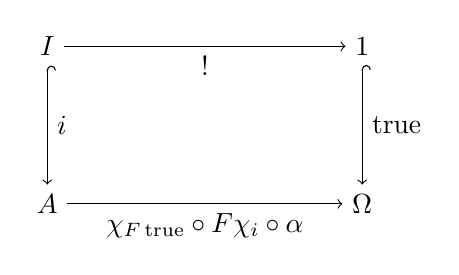
\begin{tikzpicture}[auto,every node/.style={on grid,node distance=2cm}]
    \node (A) {$A$};
    \node[above of=A] (I) {$I$};
    \node[right=4cm of A] (Omega) {$\Omega$};
    \node[above of=Omega] (One) {$1$};
    \draw[right hook->] (I) -- node {$i$} (A);
    \draw[right hook->] (One) -- node {$\true$} (Omega);
    \draw[->] (A) -- node[swap] {$\chi_{F\true} \circ F\chi_i \circ \alpha$} (Omega);
    \draw[->] (I) -- node[swap] {$!$} (One);
  \end{tikzpicture} \\
  である。

  ところで、これは $\chi_i$ を定義する図式である \\
  \begin{tikzpicture}[auto,every node/.style={on grid,node distance=2cm}]
    \node (A) {$A$};
    \node[above of=A] (I) {$I$};
    \node[right=4cm of A] (Omega) {$\Omega$};
    \node[above of=Omega] (One) {$1$};
    \draw[right hook->] (I) -- node {$i$} (A);
    \draw[right hook->] (One) -- node {$\true$} (Omega);
    \draw[->] (A) -- node[swap] {$\chi_i$} (Omega);
    \draw[->] (I) -- node[swap] {$!$} (One);
  \end{tikzpicture} \\
  に他ならない。したがって、 $\chi_i$ の唯一性から、 $\chi_{F\true} \circ F\chi_i \circ \alpha = \chi_i$ \\
  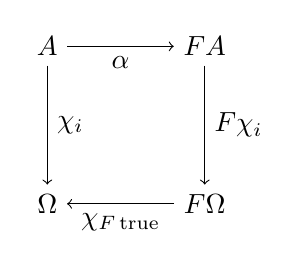
\begin{tikzpicture}[auto,every node/.style={on grid,node distance=2cm}]
    \node (A) {$A$};
    \node[right of=A] (FA) {$FA$};
    \node[below of=A] (Omega) {$\Omega$};
    \node[right of=Omega] (FOmega) {$F\Omega$};
    \draw[->] (A) -- node {$\chi_i$} (Omega);
    \draw[->] (FA) -- node {$F\chi_i$} (FOmega);
    \draw[->] (A) -- node[swap] {$\alpha$} (FA);
    \draw[->] (FOmega) -- node {$\chi_{F\true}$} (Omega);
  \end{tikzpicture} \\
  がわかる。これは $\chi_i$ が余代数-代数準同型であることを意味している。

  一方、以下の図式 \\
  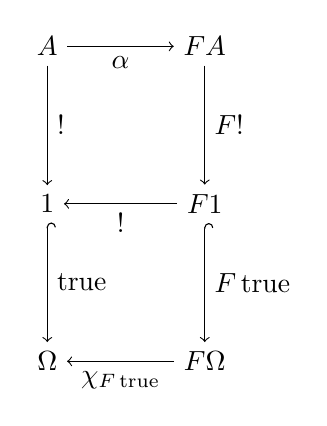
\begin{tikzpicture}[auto,every node/.style={on grid,node distance=2cm}]
    \node (A) {$A$};
    \node[right of=A] (FA) {$FA$};
    \node[below of=A] (One) {$1$};
    \node[right of=One] (FOne) {$F1$};
    \node[below of=One] (Omega) {$\Omega$};
    \node[right of=Omega] (FOmega) {$F\Omega$};
    \draw[->] (A) -- node {$!$} (One);
    \draw[right hook->] (One) -- node {$\true$} (Omega);
    \draw[->] (FA) -- node {$F!$} (FOne);
    \draw[right hook->] (FOne) -- node {$F\true$} (FOmega);
    \draw[->] (A) -- node[swap] {$\alpha$} (FA);
    \draw[->] (FOne) -- node {$!$} (One);
    \draw[->] (FOmega) -- node {$\chi_{F\true}$} (Omega);
  \end{tikzpicture} \\
  も可換となるため、 $\true \circ !$ もまた余代数-代数準同型である。

  $(A, \alpha)$ は再帰的余代数だから、 $\true \circ ! = \chi_i$ である。

  つまり、 $\chi_i$ の引き戻し図式は、以下の図式 \\
  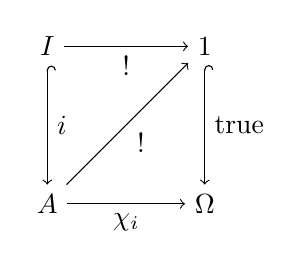
\begin{tikzpicture}[auto,every node/.style={on grid,node distance=2cm}]
    \node (A) {$A$};
    \node[above of=A] (I) {$I$};
    \node[right of=A] (Omega) {$\Omega$};
    \node[above of=Omega] (One) {$1$};
    \draw[right hook->] (I) -- node {$i$} (A);
    \draw[right hook->] (One) -- node {$\true$} (Omega);
    \draw[->] (A) -- node[swap] {$\chi_i$} (Omega);
    \draw[->] (I) -- node[swap] {$!$} (One);
    \draw[->] (A) -- node[swap] {$!$} (One);
  \end{tikzpicture} \\
  のように縮退する。 $A$ が錐をなすことを使えば、 $i$ が可逆であることがすぐにわかる。

  $i$ が可逆であることから、 $(I, i)$ は $\Sub(A)$ の最大元であることがわかった。

  ここで、$(A, \alpha)$ が整礎であることを示すために、 $(I', i')$ を帰納的な部分対象とする。 $(I', i')$ が帰納的であるというのは、言い換えると、これが $\Sub(A)$ 内で $\nexttime$ の前不動点になっていることに他ならない。

  ところで、 $(I, i)$ は最小不動点だったから、 $(I, i) \leq (I', i')$ である。したがって $(I', i')$ もまた $\Sub(A)$ の最大元である。言い換えれば、 $i'$ は可逆である。

  以上により、 $(A, \alpha)$ が整礎であることが示された。
\end{proof}

\bibliographystyle{plain}
\bibliography{refs}

\end{document}

